\documentclass[a4paper,12pt]{article}

\usepackage[utf8]{inputenc}
\usepackage{polski}
\usepackage{a4wide}

\usepackage[colorlinks=true,linkcolor=blue,urlcolor=blue]{hyperref}

\usepackage[pdftex]{graphicx}



\hypersetup{
	unicode = true,
	pdfauthor = {Daniel Kłobuszewski, Jan Stępień},
}

\title{Cumulonimbus -- Architektura Systemu}
\author{Daniel Kłobuszewski, Jan Stępień}

\def\cb{Cumulonimbus}
\def\todo{\textbf{TODO}: }

\begin{document}

\maketitle

\section{Swift}

Do realizacji projektu \cb{} wykorzystany został projekt OpenStack Storage, znany
również jako Swift. Wyczerpujący opis tego narzędzia znajduje się w~jednym
z~dokumentów dostarczonych na początku semestru \cite{qba-swift}, stąd
w~niniejszym dokumencie nie będziemy zajmować się szczegółami jego działania.
Ograniczamy się jedynie do przypomnienia, że Swift to rozproszony system
bazodanowy pozwalający na redundancyjne przechowywanie plików w~kontenerach
o~płaskiej strukturze.

\subsection{Konfiguracja}

Projekt \cb{} wymaga do swojego działania dostępu do działającego klastra Swift
o~dowolnej architekturze. Prace deweloperskie były prowadzone na minimalnej
instancji uruchomionej na pojedynczej maszynie wirtualnej. Testy w~laboratorium
wykonywano na bardziej rozbudowanej instalacji z~serwerami danych rozproszonymi
na kilku maszynach fizycznych. \todo oby to była prawda.

Sposób konfiguracji minimalnej instancji Swift potrzebnej do działania projektu
\cb{} -- Swift All In One -- został przedstawiony w~dokumentacji Swift
\cite{swift_doc}. Rozwiązanie to powoduje uruchomienie serwera autoryzującego,
serwera pośredniczącego oraz czterech serwerów danych na jednej maszynie
fizycznej. Alternatywne rozwiązania umożliwiają uruchomienie każdego
z~powyższych serwerów na różnych maszynach fizycznych, co nadaje całemu
rozwiązaniu cechy systemów \textit{fault-tolerant}.

\subsection{Zalety}

Projekt \cb{} jest niezależny od sposobu konfiguracji klastra Swift. Może być to
zarówno minimalna instancja uruchomiona na pojedynczej maszynie fizycznej, jak
i~rozproszony system wielu instancji. Dzięki poziomowi przezroczystości
zapewnianej przez Swift sposób jego instalacji nie ma znaczenia dla projektu
\cb{}. Przezroczystość ta pozwala projektowi \cb{} na udostępnienie
użytkownikowi systemu plików o~szeregu zalet.

Po pierwsze, Swift gwarantuje redundancyjne mechanizmy przechowywania danych
oraz \textit{fault-tolerance}. W~wypadku uszkodzenia pewnej części węzłów
klastra przechowujących dane system plików \cb{} może nadal działać poprawnie,
pod warunkiem, że awaria nie zaburzy działania samego systemu Swift. Jeżeli
zapewnieni autorów Swift są poprawne, użytkownik nie powinien odczuć żadnych
konsekwencji tego typu zdarzeń.

Drugą zaletą jest możliwość złączenia w~ramach klastra Swift dowolnie dużej
przestrzeni dyskowej. W~efekcie \cb{} pozwala na przechowywanie wielkiej ilości
danych, które zostaną automatycznie rozlokowane pomiędzy dyskami wchodzącymi
w~skład maszyn tworzących wykorzystywany przez \cb{} klaster.

Trzecią zaletą jest wysoki poziom abstrakcji interfejsu Swift, który udostępnia
jedynie podstawowe funkcje odpowiadające za mechanizmy przechowywania
i~odzyskiwania danych. Mechanizmy redundancyjnego rozmieszczania danych
w~klastrze, wydajnego wyszukiwania obiektów potrzebnych do zrealizowania żądania
użytkownika czy też zapewnienie spójności pomiędzy serwerami danych jest
dokonywane automatycznie. Jako autorzy systemu plików nie musimy też rozwiązywać
skomplikowanego zagadnienia jakim jest fragmentacja partycji.

\section{FUSE}

\begin{figure}
	\centering
	\includegraphics[width=0.6\textwidth]{fuse.pdf}
	\caption{Architektura systemu}
	\label{fig:fuse}
\end{figure}

W~systemie operacyjnym Linux systemy plików implementowane są i~działają w
przestrzeni adresowej jądra. Istnieje jednak możliwość implementacji takiego
systemu w~przestrzeni użytkownika. Pozwala na to biblioteka FUSE -- Filesystem
in Userspace. Odpowiada ona za przekazywanie niskopoziomowych wywołań systemu
plików do procesu użytkownika.

Dzięki temu możliwa jest implementacja pełnoprawnego systemu plików bez
jakiejkolwiek ingerencji w~kod jądra. Niewątpliwą wygodą tego rozwiązania
jest fakt, że żaden błąd w~takiej implementacji nie może zakłócić działania
jądra systemu -- inaczej niż w~tradycyjnych systemach plików.

Kolejną zaletą tej biblioteki jest obecność bindingów do różnych języków
programowania, w~tym do Pythona, na którego użycie się zdecydowaliśmy.

\begin{figure}
    \centering
    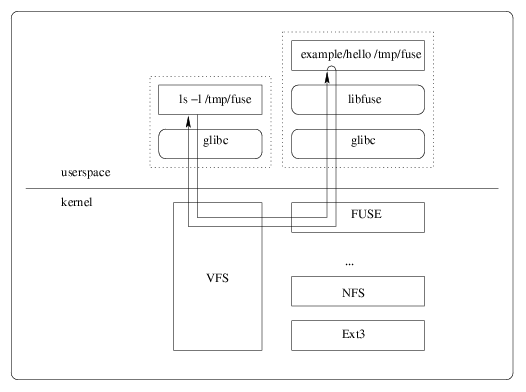
\includegraphics[width=0.7\textwidth]{img/fuse_structure.png}
    \caption{Zasada działania FUSE}
\end{figure}

\section{Instrukcja obsługi}
Użycie naszego projektu różni się jedynie sposobem montowania i~demontowania
systemu plików. Cała reszta poleceń powłoki i~wywołań I/O~jest identyczna.

\subsection{Montowanie}

Aby zamontować system plików używamy polecenia:

\begin{verbatim}
./cfuse.py <mountpoint> <opcje>
\end{verbatim}

Opcje wbrew nazwie nie są opcjonalne. Pierwsza z~nich to authurl -- adres URL
serwera autoryzacji. Kolejne dwie to user oraz key -- czyli użytkownik oraz
jego hasło na tym serwerze.

Opcje podajemy po fladze -o:

\begin{verbatim}
./cfuse.py dir -o~authurl=http://127.0.0.1:8080/auth/v1.0 \
    -o~user=test:tester -o~key=testing
\end{verbatim}

Warto zwrócić uwagę na charakterystyczny dwukropek w~nazwie użytkownika.
Oddziela on pierwszy człon nazwy -- konto -- od drugiego -- faktycznej nazwy.
Na jednym koncie może znajdować się wielu użytkowników, każdy z~innymi
uprawnieniami.

\subsection{Demontowanie}

Demontowanie jest na szczęście znacznie prostsze:

\begin{verbatim}
fusermount -u~<mountpoint>
\end{verbatim}

\bibliographystyle{../plplainurl}
\bibliography{../bibliografia}

\end{document}
